\documentclass[10pt, a5paper]{article}
\usepackage{pdfpages}
\usepackage{parallel}
\usepackage[T2A]{fontenc}
\usepackage{ucs}
\usepackage[utf8x]{inputenc}
\usepackage[polish,english,russian]{babel}
\usepackage{hyperref}
\usepackage{rotating}
\usepackage[inner=2cm,top=1.8cm,outer=2cm,bottom=2.3cm,nohead]{geometry}
\usepackage{listings}
\usepackage{graphicx}
\usepackage{wrapfig}
\usepackage{longtable}
\usepackage{indentfirst}
\usepackage{array}
\newcolumntype{P}[1]{>{\raggedright\arraybackslash}p{#1}}
\frenchspacing
\usepackage{fixltx2e} %text sub- and superscripts
\usepackage{icomma} % коскі ў матэматычным рэжыме
\PreloadUnicodePage{4}

\newcommand{\longpage}{\enlargethispage{\baselineskip}}
\newcommand{\shortpage}{\enlargethispage{-\baselineskip}}

\def\switchlang#1{\expandafter\csname switchlang#1\endcsname}
\def\switchlangbe{
\let\saverefname=\refname%
\def\refname{Літаратура}%
\def\figurename{Іл.}%
}
\def\switchlangen{
\let\saverefname=\refname%
\def\refname{References}%
\def\figurename{Fig.}%
}
\def\switchlangru{
\let\saverefname=\refname%
\let\savefigurename=\figurename%
\def\refname{Литература}%
\def\figurename{Рис.}%
}

\hyphenation{admi-ni-stra-tive}
\hyphenation{ex-pe-ri-ence}
\hyphenation{fle-xi-bi-li-ty}
\hyphenation{Py-thon}
\hyphenation{ma-the-ma-ti-cal}
\hyphenation{re-ported}
\hyphenation{imp-le-menta-tions}
\hyphenation{pro-vides}
\hyphenation{en-gi-neering}
\hyphenation{com-pa-ti-bi-li-ty}
\hyphenation{im-pos-sible}
\hyphenation{desk-top}
\hyphenation{elec-tro-nic}
\hyphenation{com-pa-ny}
\hyphenation{de-ve-lop-ment}
\hyphenation{de-ve-loping}
\hyphenation{de-ve-lop}
\hyphenation{da-ta-ba-se}
\hyphenation{plat-forms}
\hyphenation{or-ga-ni-za-tion}
\hyphenation{pro-gramming}
\hyphenation{in-stru-ments}
\hyphenation{Li-nux}
\hyphenation{sour-ce}
\hyphenation{en-vi-ron-ment}
\hyphenation{Te-le-pathy}
\hyphenation{Li-nux-ov-ka}
\hyphenation{Open-BSD}
\hyphenation{Free-BSD}
\hyphenation{men-ti-on-ed}
\hyphenation{app-li-ca-tion}

\def\progref!#1!{\texttt{#1}}
\renewcommand{\arraystretch}{2} %Іначай формулы ў матрыцы зліпаюцца з лініямі
\usepackage{array}

\def\interview #1 (#2), #3, #4, #5\par{

\section[#1, #3, #4]{#1 -- #3, #4}
\def\qname{LVEE}
\def\aname{#1}
\def\q ##1\par{{\noindent \bf \qname: ##1 }\par}
\def\a{{\noindent \bf \aname: } \def\qname{L}\def\aname{#2}}
}

\def\interview* #1 (#2), #3, #4, #5\par{

\section*{#1\\{\small\rm #3, #4. #5}}

\def\qname{LVEE}
\def\aname{#1}
\def\q ##1\par{{\noindent \bf \qname: ##1 }\par}
\def\a{{\noindent \bf \aname: } \def\qname{L}\def\aname{#2}}
}

\begin{document}
\title{Эффективная разработка и сопровождение Ansible-ролей\footnote{\url{other.bigmouse@gmail.com}, \url{https://lvee.org/en/abstracts/277}}}
\author{Aliaksandr Kharkevich, Gomel, Belarus}
\maketitle
\begin{abstract}
In case of using different SCM the most important aspects are: correct work of target configuration, simplicity lifecycle support of DSL code written for target SCM and having different tests for things which is under control of SCM.
This article shows more efficient way for development, testing and support for Ansible-roles; including continuous integration, code-review, guideline compliance.
\end{abstract}
\subsection*{Глоссарий}

\textbf{Ansible}~--- система управления конфигурациями, написанная на Python, с использованием декларативного языка разметки для описания конфигураций.
\textbf{Molecule}~--- программное обеспечение (ПО), созданное для разработки и тестирования Ansible ролей в различных средах.
\textbf{Ansible Galaxy}~--- вебсайт, где пользователи могут публиковать роли для совместного использования, а также инструмент командной строки для установки, создания и управления ролями.
\textbf{GitHub, GitLab}~--- сайт и система управления репозиториями кода для Git.
\textbf{GitLab Runner}~--- часть GitLab проекта, используемая для процессов непрерывной интеграции и непрерывной доставки.
\textbf{Travis-CI}~--- веб-сервис для сборки и тестирования различного программного обеспечения, использующий GitHub в качестве хостинга исходного кода.

\subsection*{Введение}

На сегодняшний день, использование систем управления конфигурациями~--- это наиболее эффективный путь для упрощения процесса управления состояниям на целевой системе. Одной из задач конфигурационного управления можно назвать ответ на вопрос: <<Произошло какое-то изменение, как это воспроизвести?>>. На текущий момент одной из наиболее известных систем управления конфигурациями является Ansible.
Ansible обладает следующими критериями:

\begin{itemize}
  \item Низкий порог вхождения
  \item Обширная документация
  \item Простота расширения сторонними модулями
  \item Отсутствие агентов на конечных машинах
  \item YAML в качестве DSL
\end{itemize}

\subsection*{Ansible и повторное использование кода}

Так называемые роли~--- родной механизм для повторного использования кодовой базы. Роль представляет собой отдельно выделенный, самостоятельный фрагмент кода, который приведет целевую систему в ожидаемое состояние.
Galaxy веб-сайт (\url{https://galaxy.ansible.com}) представляет собой витрину готовых ролей, уже разработанных кем-либо.
Ansible роль может быть как импортирована с galaxy (ansible-galaxy install \textless{}имя\_разработчика\textgreater{}.\textless{}название\_роли\textgreater{}) так и создана с нуля (ansible-galaxy init).
Типовая структура роли, созданной при помощи ansible-galaxy


\begin{figure}[h!]
  \centering
  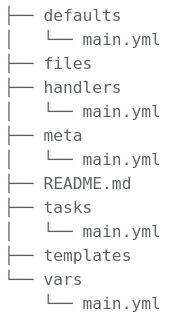
\includegraphics[width=3cm]{05_2018_Kharkevich6.png}
  %\caption{}
  \label{Kharkevich1}
\end{figure}

В рамках данной структуры и описываются все необходимые действия по приведению части системы в ожидаемое состояние.
После финализации данной роли можно осуществить публикацию её на GitHub с последующим импортом в ansible-galaxy. Но при такой упрощенной системе публикации нет никакого процесса контроля качества данной роли.

\subsection*{Соответствие стилевым рекомендациям}

Одним из самых простых механизмов проверки качества кода является использование статического анализатора кода. Наиболее эффективными инструментами для Ansible являются:

\begin{itemize}
  \item yamllint (\url{https://pypi.org/project/yamllint/})
  \item ansible-lint (\url{https://pypi.org/project/ansible-lint/})
\end{itemize}

Последний, в свою очередь, может использовать как встроенный, так и подключаемый список правил.
Кроме того, данные статические анализаторы могут быть встроены в различные системы непрерывной интеграции для предотвращения попадания кода, несоответствующего требованиям.

\subsection*{Платформа для тестирования}

Для тестирования Ansible ролей, на сегодняшний день, molecule является наиболее удобным инструментом. Который, в свою очередь поддерживает множественные интеграции с различными средами, которые могут выступать в роли целевых платформ; такие как: Docker, AWS, Microsoft Azure, Google Cloud Platform и др.
Интегрировать molecule-тесты можно в любой момент, выполнив инициализацию нового тестового сценария (molecule init scenario -r \textless{}имя\_роли\textgreater{}). После данной инициализации будет создана структура для тестов с параметрами по умолчанию (galaxy~--- для решения зависимостей, docker~--- как целевая платформа для разворачивания тестовой среды, default~--- как имя тестового сценария, testinfra~--- как тестовый фреймворк для проведения интеграционных тестов).
Типовая структура роли после инициализации тестового сценария molecule:
\newpage
\begin{figure}[h!]
  \centering
  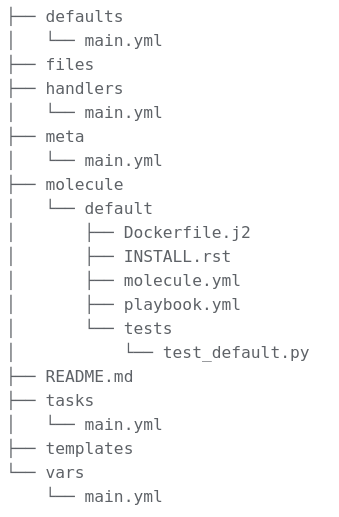
\includegraphics[width=5cm]{05_2018_Kharkevich5.png}
  %\caption{}
  \label{Kharkevich2}
\end{figure}


Без какого-либо дополнительного вмешательства, стразу после инициализации, данный тест готов проверить вашу роль на статический анализ, успешность применения в тестовой среде и идемпотентность.
Для поддержания качества разрабатываемой роли в требуемом состоянии необходимо подключить какую-либо из систем непрерывной интеграции.

\subsection*{Непрерывная интеграция (CI)}

Travis-CI является одной из самых доступных систем непрерывной интеграции для проектов с открытым исходным кодом. Для подключения данной системы достаточно просто разместить файл .travis.yml в корне репозитория и активировать CI на веб-сайте \url{https://travis-ci.org}

\begin{center}
\begin{figure}[h!]
  \centering
  
\includegraphics[width=5cm]{05_2018_Kharkevich1.png}
  %\caption{Блок-схема примерной системы распознавания РОГ}
  \label{Kharkevich3}
\end{figure}
\end{center} 
Содержимое .travis.yml файла для вышеописанной роли может быть следующем:

\begin{verbatim}
---
dist: xenial
sudo: required
language: python
python:
  - "2.7"
services:
  - docker
before_install:
  - git clone -b ${lint_version} https://github.com/
lean-delivery/ansible-lint-rules.git ~/ansible-lint-rules
install:
  - pip install --upgrade ansible==2.5.5 ansible-lint==3.4.21 
docker-py==1.10.6 molecule==2.13.1 pyOpenSSL PyYAML==3.12
  - ansible --version
  - molecule --version
script:
  - ansible-lint -c .ansible-lint `find . -regex ".*\.\(yml\)"`
  - molecule test
notifications:
  webhooks: https://galaxy.ansible.com/api/v1/notifications/\end{verbatim}
После активации CI при последующем изменении кода в репозитории запустится процесс тестирования в рамках вышеописанного molecule-сценария:

\begin{center}
\begin{figure}[h!]
  \centering
  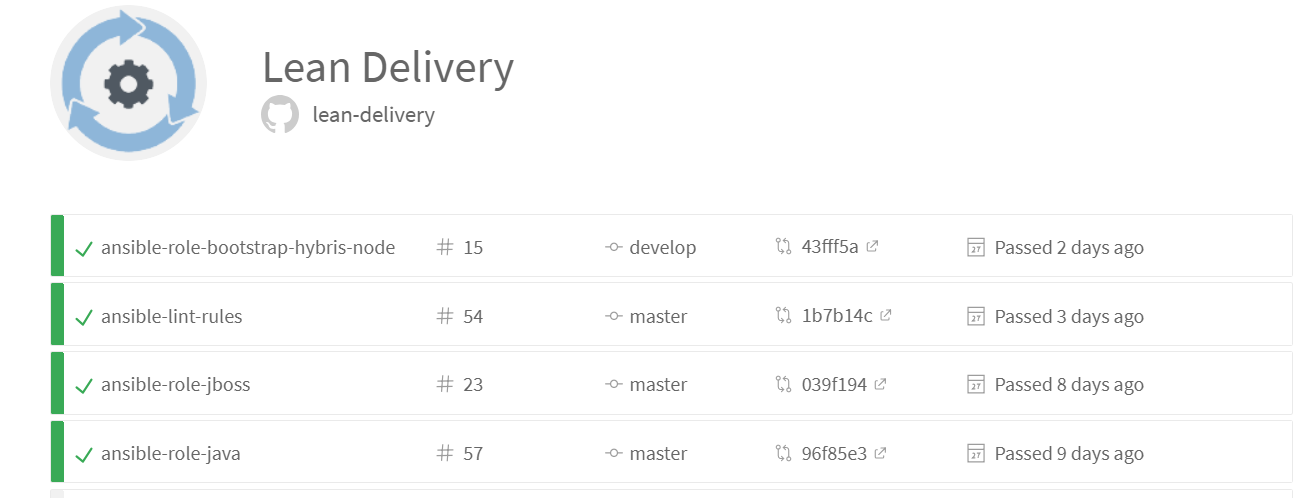
\includegraphics[width=9cm]{05_2018_Kharkevich2.png}
  %\caption{Блок-схема примерной системы распознавания РОГ}
  \label{Kharkevich4}
\end{figure}
\end{center} 

Иногда бывает необходимо проводить тестирование в непубличных средах. Например, вы хотите провести тестирование не только в докере, но и в других облачных сервисах, при этом вы хотите препятствовать утечке API ключа, который понадобится для запуска тестовых сред. В этом случае можно использовать немного более сложную топологию интеграции и подключить GitLab CI к GitHub репозиториям.
Для этого вам необходимо на веб-сайте \url{https://gitlab.com} подключить ваш GitHub репозиторий как “CI/CD for external repo”. После этого у вас появится зеркало вашего репозитория, цель которого лишь запускать ваш код на сборку и тестирование, руководствуясь инструкциями из файла .gitlab-ci.yml. В данном случае CI топология будет аналогична CI с использованием Travis-CI, за исключением возможности подключения GitLab Runner, который размещается в вашей приватной сети (возможность использовать публичные GitLab Runner остаётся). 

\begin{center}
\begin{figure}[h!]
  \centering
  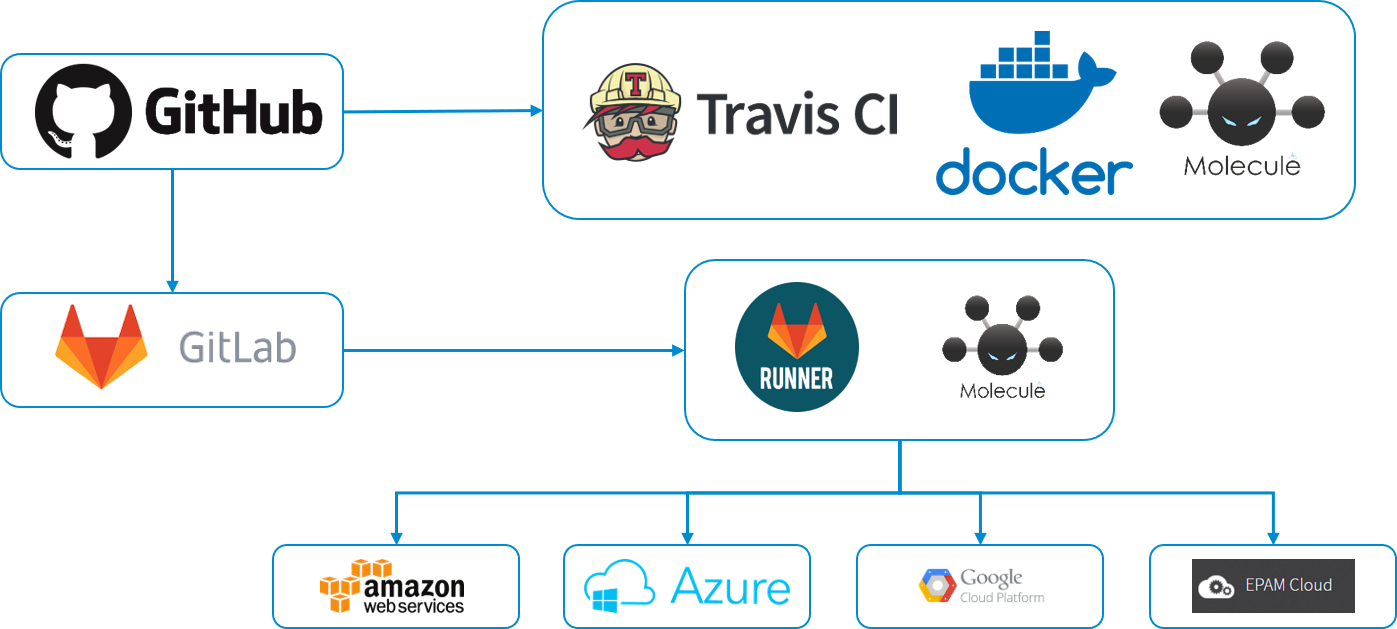
\includegraphics[width=5cm]{05_2018_Kharkevich3.png}
  %\caption{Блок-схема примерной системы распознавания РОГ}
  \label{Kharkevich5}
\end{figure}
\end{center} 

\subsection*{Вместо заключения}

\begin{center}
\begin{figure}[h!]
  \centering
  
\includegraphics[width=9cm]{05_2018_Kharkevich4.png}
  %\caption{Блок-схема примерной системы распознавания РОГ}
  \label{Kharkevich6}
\end{figure}
\end{center} 

Интегрировав данные инструменты в рамках процесса тестирования Ansible ролей, мы получили достаточно простой, но тем не менее эффективный инструмент, позволяющий поддерживать нашу кодовую базу в единообразном состоянии и быть уверенными в том, что данные роли работоспособны на различных целевых платформах вне зависимости от (не)желания этому помешать.

\begin{thebibliography}{20}
  \bibitem{Kharkevich-1} Molecule \url{https://molecule.readthedocs.io}
  \bibitem{Kharkevich-2} Примеры Ansible ролей \url{https://galaxy.ansible.com/lean_delivery/}
  \bibitem{Kharkevich-3} Интеграция GitLab CI и GitHub \url{https://about.gitlab.com/features/github/}
  \bibitem{Kharkevich-4} Travis-CI \url{https://github.com/marketplace/travis-ci}
  \bibitem{Kharkevich-5} Дополнительные ansible-lint правила \url{https://github.com/lean-delivery/ansible-lint-rules}
\end{thebibliography}

\end{document}
